% $Header: /cvsroot/latex-beamer/latex-beamer/solutions/generic-talks/generic-ornate-15min-45min.en.tex,v 1.5 2007/01/28 20:48:23 tantau Exp $

\documentclass[12pt]{beamer}
%\documentclass[12pt,handout]{beamer}

% This file is a solution template for:

% - Giving a talk on some subject.
% - The talk is between 15min and 45min long.
% - Style is ornate.



% Copyright 2004 by Till Tantau <tantau@users.sourceforge.net>.
%
% In principle, this file can be redistributed and/or modified under
% the terms of the GNU Public License, version 2.
%
% However, this file is supposed to be a template to be modified
% for your own needs. For this reason, if you use this file as a
% template and not specifically distribute it as part of a another
% package/program, I grant the extra permission to freely copy and
% modify this file as you see fit and even to delete this copyright
% notice.


\mode<presentation>
{
  \usetheme{default}
  % or ...

  \setbeamercovered{transparent}
  % or whatever (possibly just delete it)
}
\setbeamertemplate{navigation symbols}{}%remove navigation symbols


\usepackage[english]{babel}
% or whatever

\usepackage[latin1]{inputenc}
% or whatever

\usepackage{times}
\usepackage{sansmathfonts}
\usepackage[T1]{fontenc}
% Or whatever. Note that the encoding and the font should match. If T1
% does not look nice, try deleting the line with the fontenc.


\title%[Short Paper Title] % (optional, use only with long paper titles)
{}

\subtitle
{} % (optional)

\author%[Author, Another] (optional, use only with lots of authors)
{Ben Holder}%{F.~Author\inst{1} \and S.~Another\inst{2}}
% - Use the \inst{?} command only if the authors have different
%   affiliation.

%\institute[Universities of Somewhere and Elsewhere] % (optional, but mostly needed)
%{
%  \inst{1}%
%  Department of Computer Science\\
%  University of Somewhere
%  \and
%  \inst{2}%
%  Department of Theoretical Philosophy\\
%  University of Elsewhere}
%% - Use the \inst command only if there are several affiliations.
%% - Keep it simple, no one is interested in your street address.

\date%[Short Occasion] % (optional)
{}

\subject{Talks}
% This is only inserted into the PDF information catalog. Can be left
% out.



% If you have a file called "university-logo-filename.xxx", where xxx
% is a graphic format that can be processed by latex or pdflatex,
% resp., then you can add a logo as follows:

% \pgfdeclareimage[height=0.5cm]{university-logo}{university-logo-filename}
% \logo{\pgfuseimage{university-logo}}



% Delete this, if you do not want the table of contents to pop up at
% the beginning of each subsection:
%\AtBeginSubsection[]
%{
%  \begin{frame}<beamer>{Outline}
%    \tableofcontents[currentsection,currentsubsection]
%  \end{frame}
%}


% If you wish to uncover everything in a step-wise fashion, uncomment
% the following command:

%\beamerdefaultoverlayspecification{<+->}

\usepackage{enumerate}
\usepackage{amsmath}
\usepackage{amssymb}
\usepackage[amssymb]{SIunits}
\usepackage{url}
\usepackage{hyperref}
\usepackage[normalem]{ulem}


\setbeamercovered{invisible}

\hypersetup{
    colorlinks=true,     % false: boxed links; true: colored links
    linkcolor=red,       % color of internal links
    citecolor=blue,      % color of links to bibliography
    filecolor=blue,      % color of file links
    urlcolor=blue        % color of external links
}


\begin{document}

%\begin{frame}
%  \titlepage
%\end{frame}

%%%%%%%%%%%%%%%%%%%%%%%%%%%%%%%%%%%%%%
\begin{frame}{Announcements}
	%
	\begin{itemize}
	\addtolength{\itemsep}{0.5\baselineskip}
	\item Any questions/issues?
	\item \underline{Schedule}:
		%
		\begin{itemize}
		\item[]{\bf Today (Follow-up)}: Discussion Q2 --- $T_\text{Earth}$
		\item[]{\bf Today (New)}: Milankovitch cycles --- long-time perturbations of temperature
		\item[]{\bf Tomorrow (Lab)}: clouds!
		\item[]{\bf Thursday (Discussion)}: Paleotemperatures and Milankovitch
		\item[] {\bf Next Week}: ``Climate sensitivity'' ---  $\text{CO}_2$ effect on temperature
		\end{itemize}
		%
	\end{itemize}

\end{frame}
%%%%%%%%%%%%%%%%%%%%%%%%%%%%%%%%%%%%%%%
%\begin{frame}{Today's Reading Quiz (3 min)}
%
%
%	
%\vspace{1cm}
%
%On your own sheet of paper\ldots
%
%\vspace{0.5cm}
%
%{\bf Say a few words about each: {\em atmospheric pressure}, {\em humidity of air}, {\em latent heat}.}
%
%\vspace{0.5cm}
%
%Turn in to Blackboard as scanned pdf (or image is fine).
%
%\end{frame}
%%%%%%%%%%%%%%%%%%%%%%%%%%%%%%%%%%%%%%%
%\begin{frame}{Question 2 from Discussion}
%
%\begin{center}
%
\includegraphics[width=0.55\textwidth]{images/peixoto_fig6-5_structure-water-ozone-co2.png}
%\end{center}
%
%\end{frame}
%%%%%%%%%%%%%%%%%%%%%%%%%%%%%%%%%%%%%%%
%\begin{frame}{Question 3 from Discussion}
%
%\begin{center}
%
\includegraphics[width=0.8\textwidth]{images/atmospheric-absorption-transmission_rohde_mathez-textbook_no-caption.png}
%\end{center}
%
%
%
%\end{frame}
%%%%%%%%%%%%%%%%%%%%%%%%%%%%%%%%%%%%%%
\begin{frame}{Disc 09 --- Atmosphere \& Lapse Rate}

The layers of the atmosphere:

\begin{center}
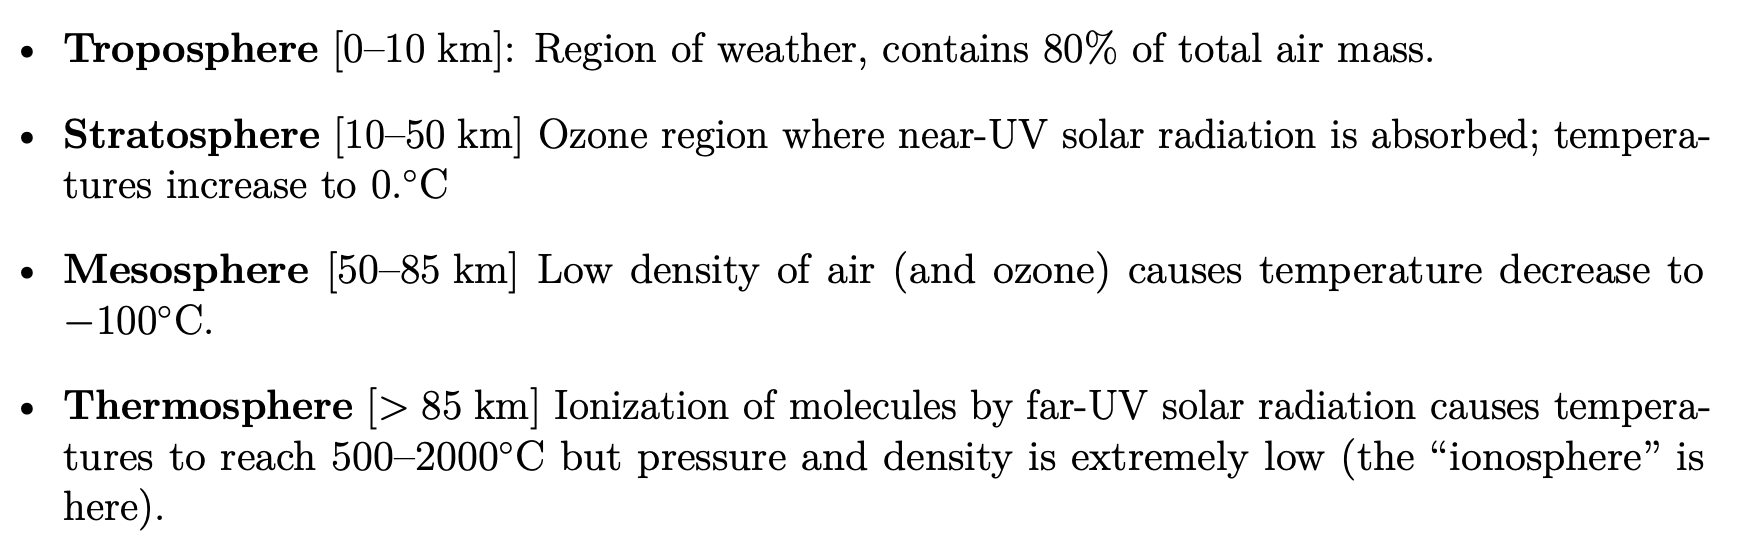
\includegraphics[width=0.9\textwidth]{images/disc09_layers-of-atmosphere.png}
\end{center}

Temperature change in the troposphere is dictated by the {\em adibatic lapse rate}:
%
\begin{equation*}
\frac{\Delta T}{\Delta h} = - \Gamma \quad \quad \text{w/} \quad \Gamma \approx 6.5 \frac{\degree\text{C}}{\text{km}}
\end{equation*}
%
which follows from  air and water vapor {\em convection}. The value above is the ``moist'' lapse rate because it includes the effect of water vapor convection; a ``dry'' lapse rate can be derived exactly from thermodynamics ($\Gamma_\text{dry} = 10 \frac{\degree\text{C}}{\text{km}}$).

\end{frame}
%%%%%%%%%%%%%%%%%%%%%%%%%%%%%%%%%%%%%%
\begin{frame}{Hurricane Melissa}


\begin{center}
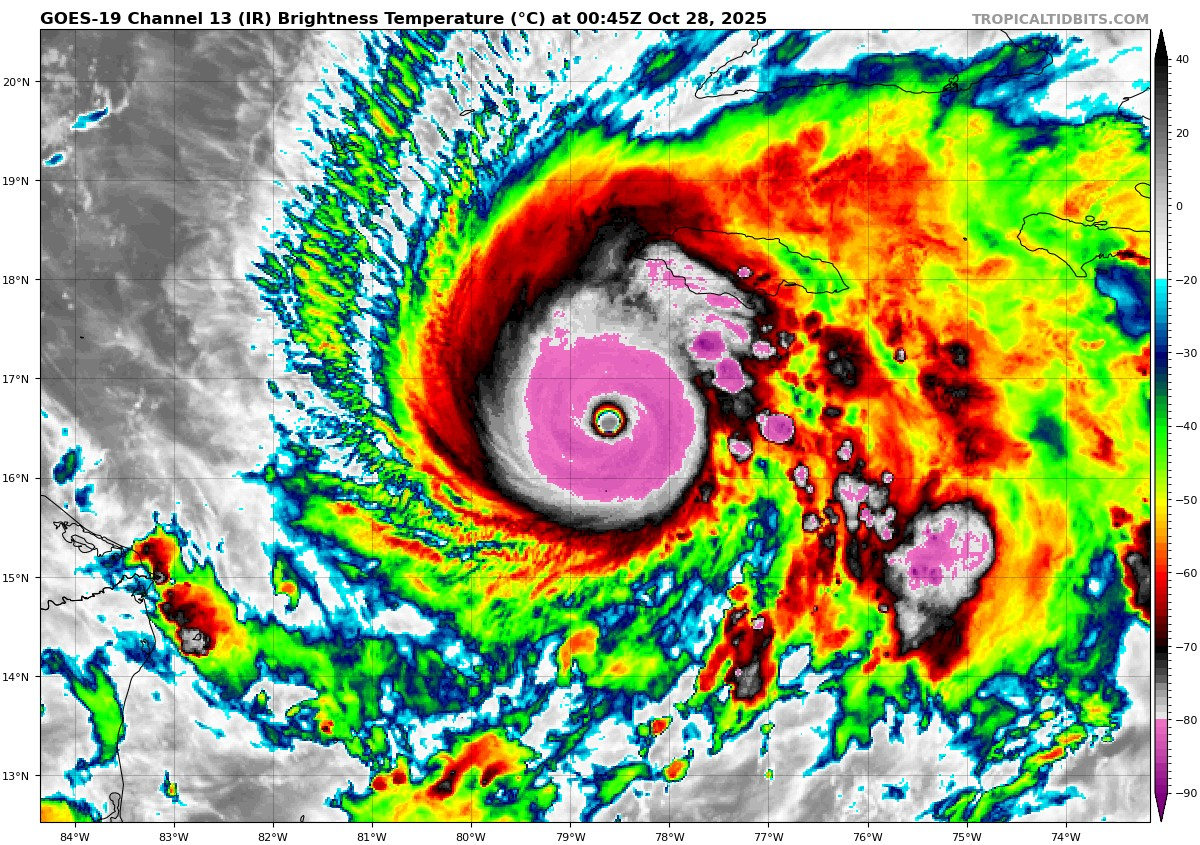
\includegraphics[width=\textwidth]{images/melissa-cold-central-hurricane.jpg}
\end{center}


\end{frame}
%%%%%%%%%%%%%%%%%%%%%%%%%%%%%%%%%%%%%%
\begin{frame}{Discussion Q2}


\begin{center}
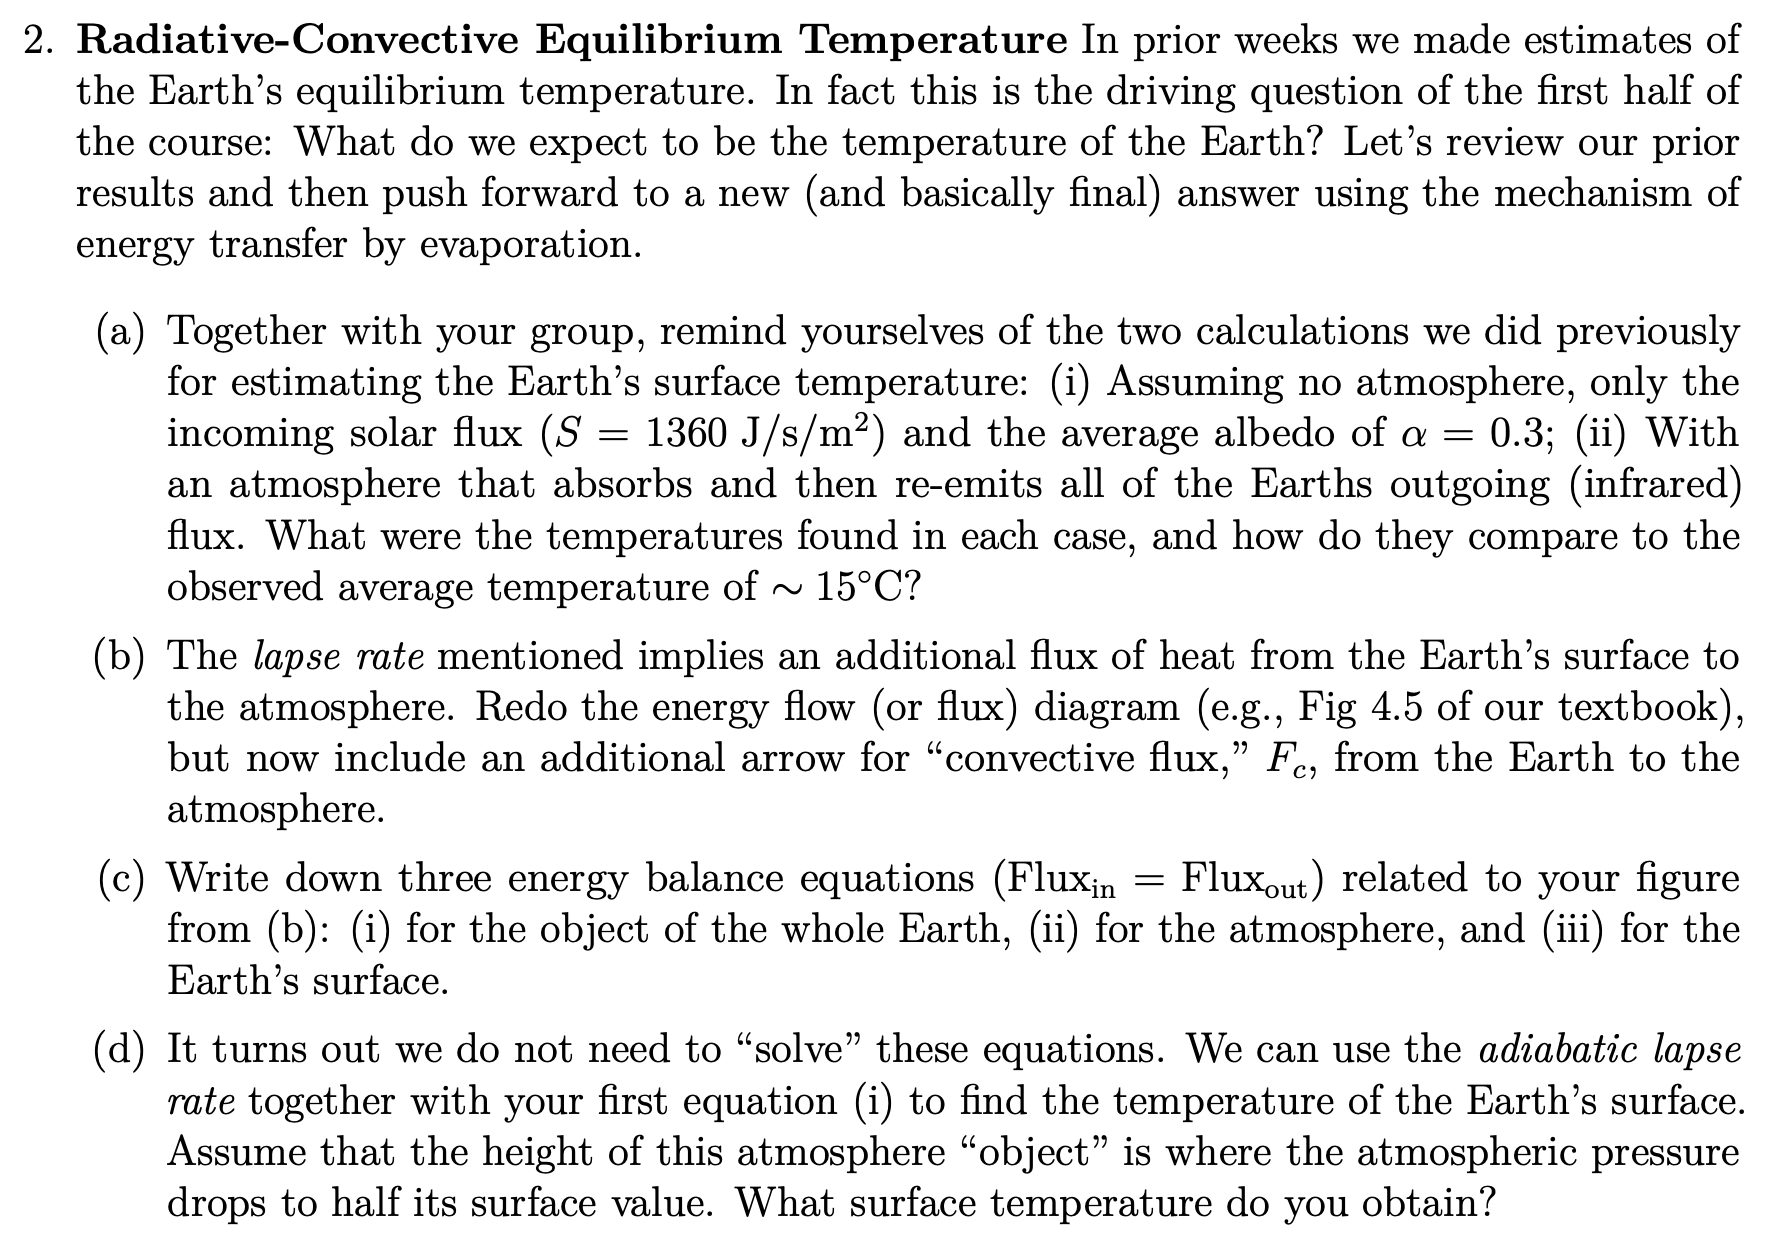
\includegraphics[width=\textwidth]{images/disc09_Q2_rad-convect-equilib-temp.png}
\end{center}


\end{frame}
%%%%%%%%%%%%%%%%%%%%%%%%%%%%%%%%%%%%%%
\begin{frame}{(i) No-atmosphere Earth}

Let's remind ourselves about our first calculation of the equilibrium temperature of the planet.  Remember that the Stefan-Boltzmann Law states
	%
	\begin{equation*}
	F = \sigma T^4 \quad \quad \text{with} \quad \sigma = 5.7 \times 10^{-8} \frac{\text{W}}{\text{m}^2 \, \text{K}^4}
	\end{equation*}
	%
and that flux means $F = \frac{\text{energy}/\text{time}}{\text{area}}$.

\vspace{7cm}


\end{frame}
%%%%%%%%%%%%%%%%%%%%%%%%%%%%%%%%%%%%%%
\begin{frame}{(ii) Earth with atmosphere}

Now consider the case where the Earth's surface is covered by an atmosphere of ideal greenhouse gases.

\vspace{7cm}


\end{frame}
%%%%%%%%%%%%%%%%%%%%%%%%%%%%%%%%%%%%%%
\begin{frame}{(b)--(c) Earth with a convective atmosphere}

As considered in the discussion, the convection of warm air --- and, most importantly, water vapor --- from the Earth's surface to the upper troposphere transports energy from the surface into the atmosphere. This gives another path of energy flux, $F_c$, which we can add to our diagram and equations.


\vspace{7cm}

\end{frame}
%%%%%%%%%%%%%%%%%%%%%%%%%%%%%%%%%%%%%%
\begin{frame}{(d) Earth with a convective atmosphere}

The solution to these equations comes simply from knowing the (moist) adiabatic lapse rate ($\Gamma = 6.5 \frac{\degree\text{C}}{\text{km}}$) and the average height of the greenhouse gas layer ($h \approx \unit{5}{\kilo\meter}$).


\vspace{7cm}


\end{frame}
%%%%%%%%%%%%%%%%%%%%%%%%%%%%%%%%%%%%%%
\begin{frame}{The Earth and Sun (and Moon)}

Let's start with some basic questions about the Earth's motion in space:
	%
	\begin{itemize}
	\item What causes day and night?
	\item What causes the seasons in the northern (or southern) hemisphere?
	\item (bonus) What causes the phases of the Moon?
	\end{itemize}


\end{frame}
%%%%%%%%%%%%%%%%%%%%%%%%%%%%%%%%%%%%%%
\begin{frame}{Seasons and eccentricity}

Currently, within a hundred-thousand-year cycle, the Earth's orbit around the Sun looks like this:
%
\begin{center}
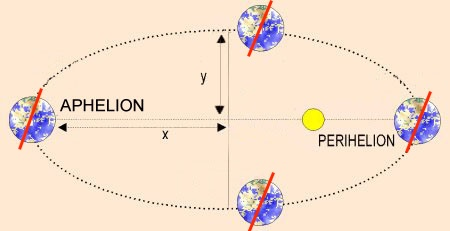
\includegraphics[width=0.7\textwidth]{images/eccentricity_beth-caissie-uaf_modified.jpg}\\
\hfill {\tiny (adapted from \href{http://ffden-2.phys.uaf.edu/212_fall2003.web.dir/Beth_Caissie/eccentricity.htm}{Beth Caissie, UAF})}
\end{center}
%
where the eccentricity (non-circular, ellipse nature of the orbit) has been exaggerated.\\[6pt]

{\bf Where on the orbit is northern hemisphere summer?}


\end{frame}
%%%%%%%%%%%%%%%%%%%%%%%%%%%%%%%%%%%%%%
\begin{frame}{Kepler and Newton: Two-body problem}

\begin{columns}

\begin{column}{0.25\textwidth}

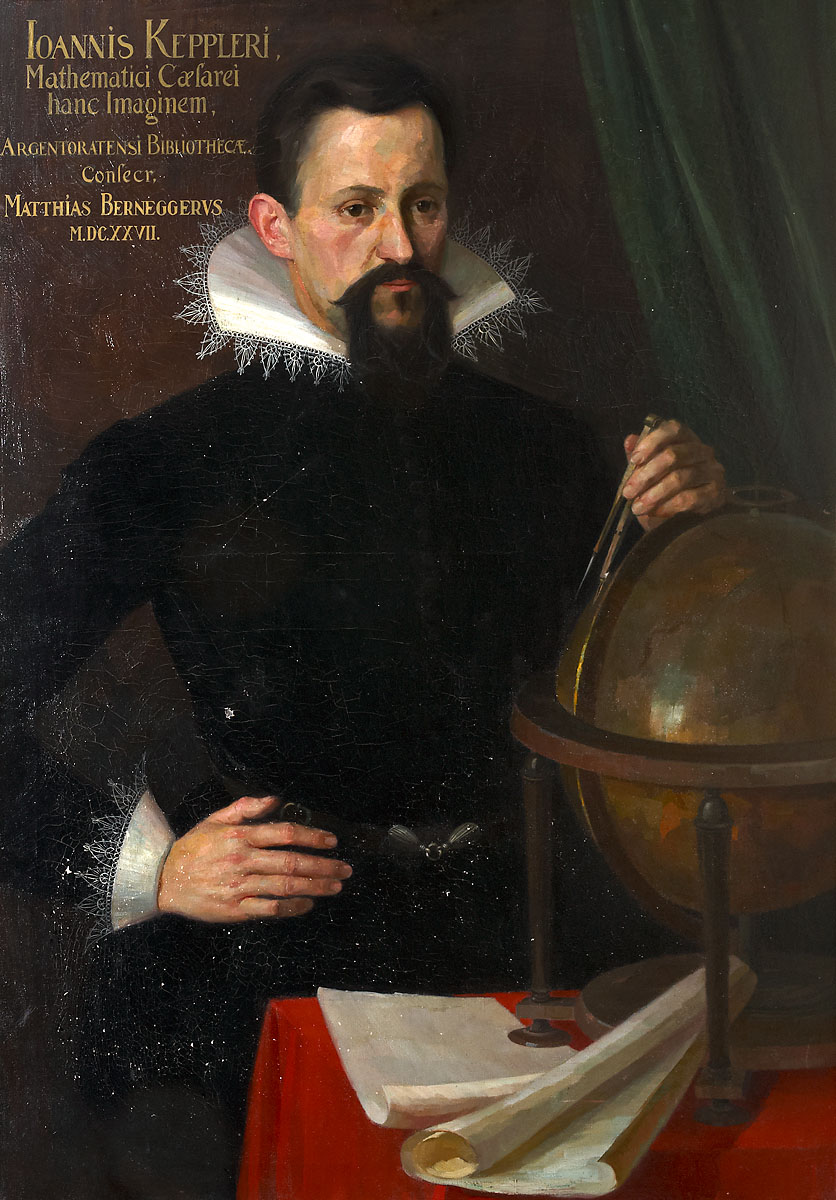
\includegraphics[width=\textwidth]{images/kepler.jpg}\\
{\tiny Kepler (1571--1630)}

\end{column}


\begin{column}{0.45\textwidth}

Johannes Kepler, using planetary data collected by Tycho Brahe, found that planets and moons follow elliptical orbits.\\[12pt]

Newton, using his dynamical law (``$F = ma$'') and his Gravitational Force ($F_G = \frac{G Mm}{r^2}$) found the theoretical origin of this observation.

\end{column}

\begin{column}{0.25\textwidth}

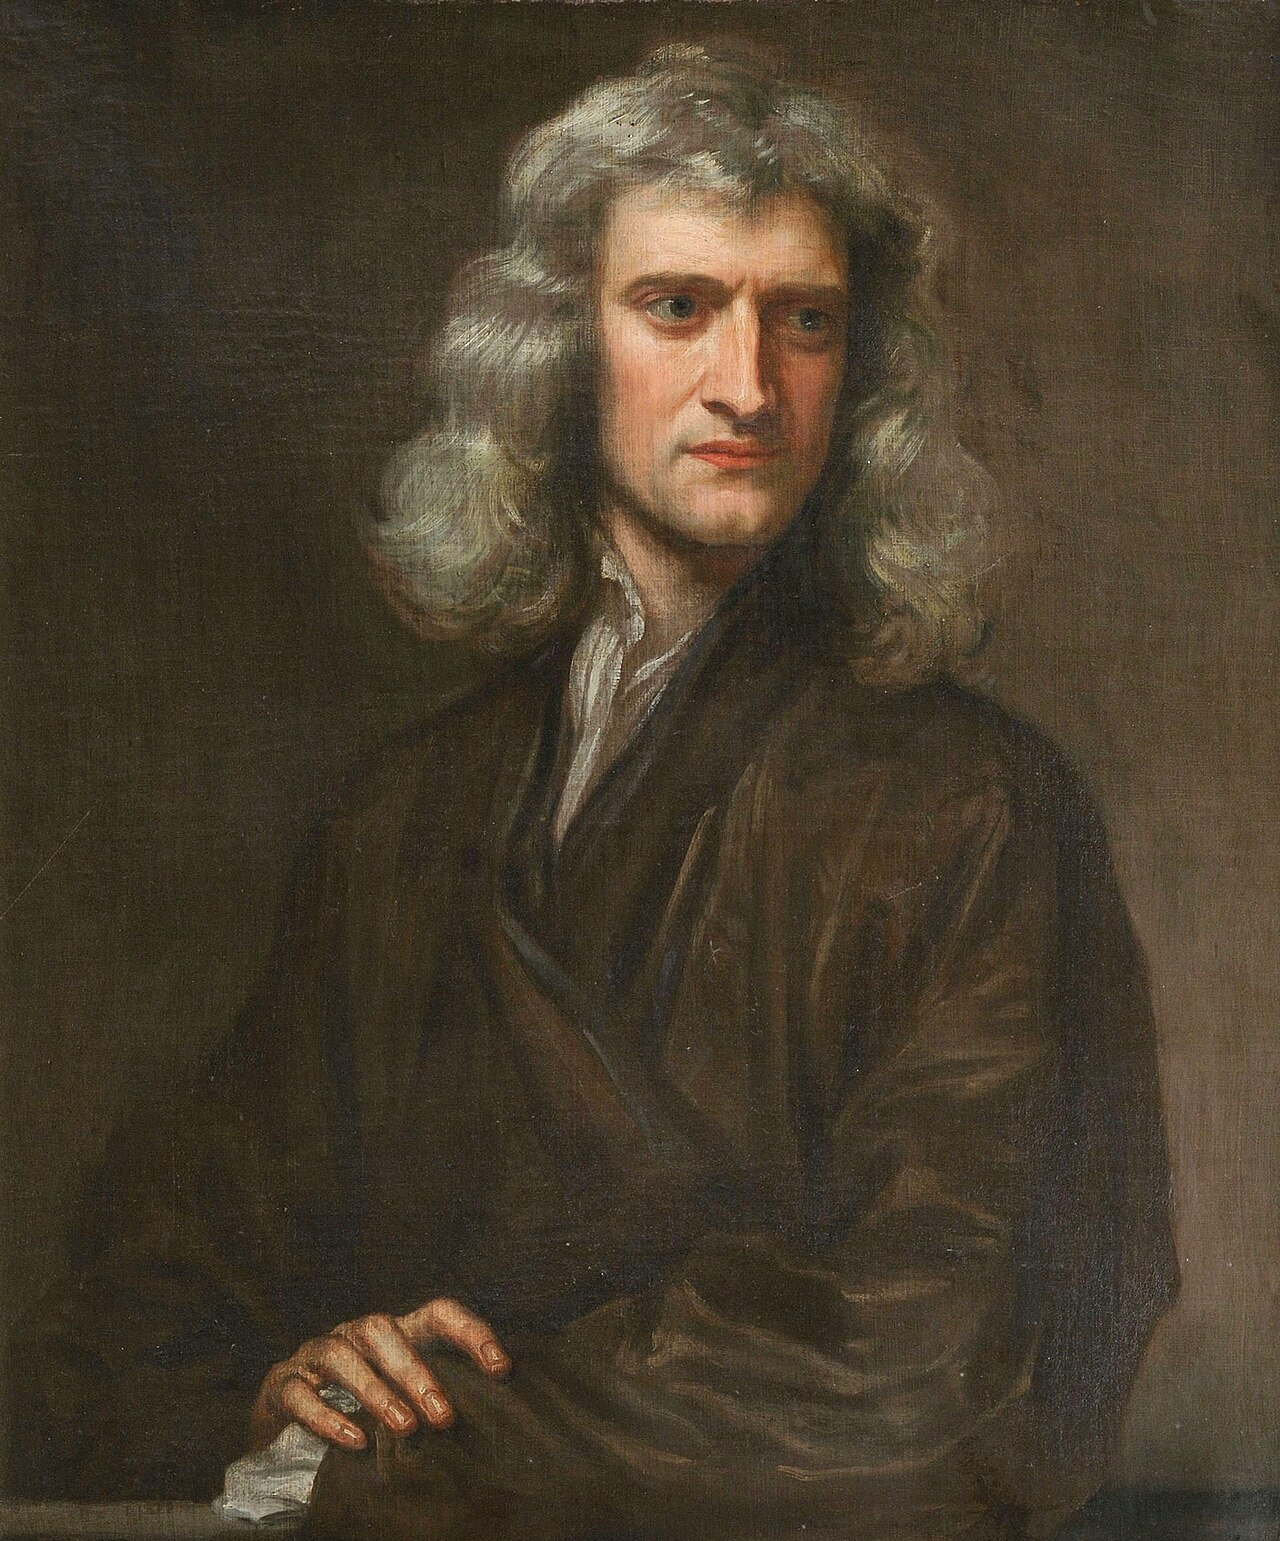
\includegraphics[width=\textwidth]{images/newton.jpg}\\
{\tiny Newton (1643--1727)}
\end{column}

\end{columns}

\vspace{0.5cm}

{\bf But when two orbiting bodies are ``perturbed'' by a third, their motion is not perfectly elliptical (the ``three-body problem'').}


\end{frame}
%%%%%%%%%%%%%%%%%%%%%%%%%%%%%%%%%%%%%%
\begin{frame}{Orbital effects on solar radiation}

The \underline{variation of eccentricity} is the the first of three orbital effects on solar radiation.

\begin{center}
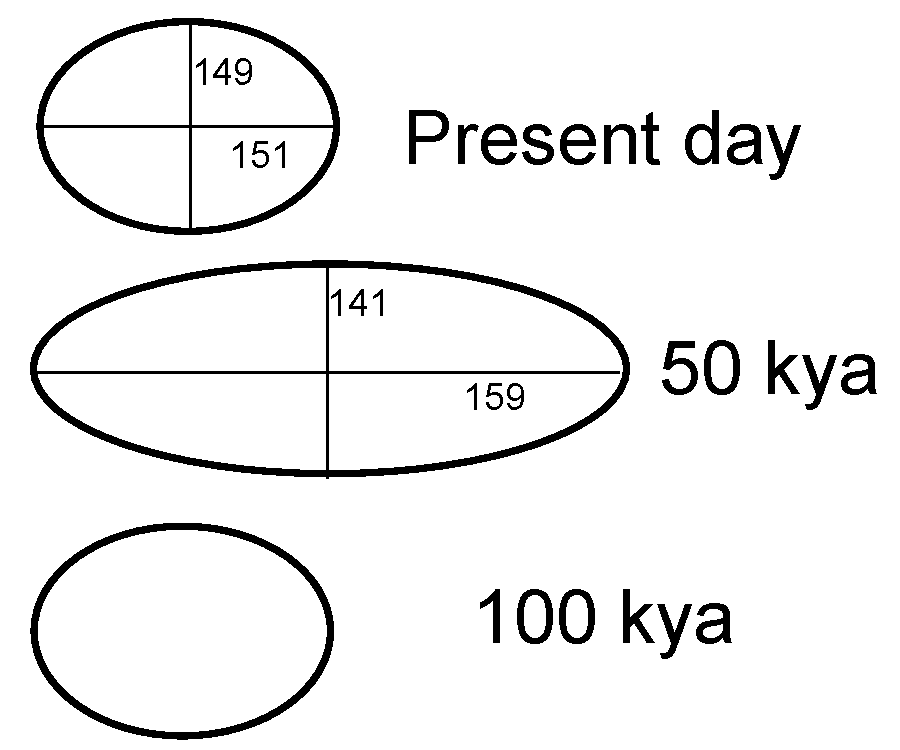
\includegraphics[width=0.8\textwidth]{images/eccentricity-changes.pdf}
\end{center}

\end{frame}
%%%%%%%%%%%%%%%%%%%%%%%%%%%%%%%%%%%%%%
\begin{frame}{Orbital effects on solar radiation}


\begin{center}
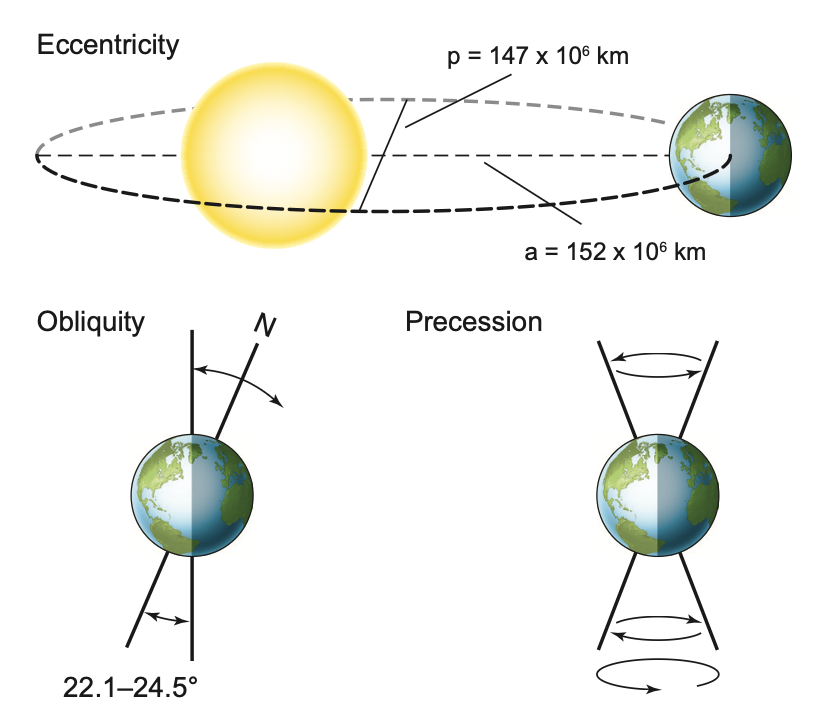
\includegraphics[width=0.8\textwidth]{images/mathez_fig7-5.png}
\end{center}

\href{https://science.nasa.gov/science-research/earth-science/milankovitch-orbital-cycles-and-their-role-in-earths-climate/}{NASA videos showing each type of change}

\end{frame}
%%%%%%%%%%%%%%%%%%%%%%%%%%%%%%%%%%%%%%
\begin{frame}{Orbital effects on solar radiation}


\begin{center}
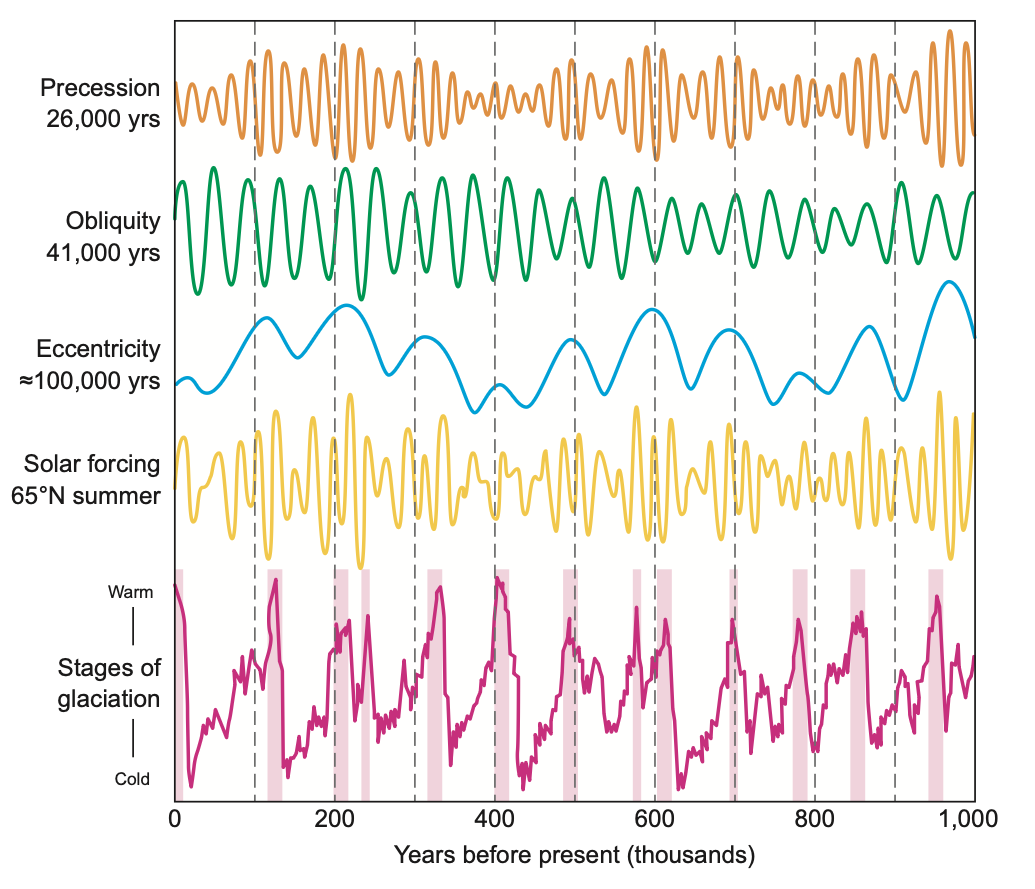
\includegraphics[width=0.8\textwidth]{images/mathez_fig7-9.png}
\end{center}

\end{frame}
%%%%%%%%%%%%%%%%%%%%%%%%%%%%%%%%%%%%%%
\end{document}
